\documentclass[9pt,a4paper,]{extarticle}

\usepackage{f1000_styles}

\usepackage[pdfborder={0 0 0}]{hyperref}

\usepackage[numbers]{natbib}
\bibliographystyle{unsrtnat}


%% maxwidth is the original width if it is less than linewidth
%% otherwise use linewidth (to make sure the graphics do not exceed the margin)
\makeatletter
\def\maxwidth{ %
  \ifdim\Gin@nat@width>\linewidth
    \linewidth
  \else
    \Gin@nat@width
  \fi
}
\makeatother


% disable code chunks background
%\renewenvironment{Shaded}{}{}

% disable section numbers
\setcounter{secnumdepth}{0}

%% added by MLS, this is not in the F1000 style by default %%

\hypersetup{unicode=true,
            pdftitle={BASiCS workflow: a step-by-step analysis of expression variability using single cell RNA sequencing data},
            pdfkeywords={Single-cell RNA sequencing, expression variability, transcriptional noise, differential expression testing},
            colorlinks=true,
            linkcolor=Maroon,
            citecolor=Blue,
            urlcolor=Orange,
            breaklinks=true}

%% End added by MLS %%

\setlength{\parindent}{0pt}
\setlength{\parskip}{6pt plus 2pt minus 1pt}



\begin{document}
\pagestyle{front}

\title{BASiCS workflow: a step-by-step analysis of expression variability using single cell RNA sequencing data}

\author[1,2]{Nils Eling\thanks{\ttfamily eling@ebi.ac.uk}}
\author[3]{Alan O'Callaghan}
\author[1,2]{John C. Marioni}
\author[3,4]{Catalina A. Vallejos\thanks{\ttfamily catalina.vallejos@igmm.ed.ac.uk}}
\affil[1]{European Molecular Biology Laboratory, European Bioinformatics Institute, Wellcome Trust Genome Campus, Hinxton, Cambridge CB10 1SD, UK}
\affil[2]{Cancer Research UK Cambridge Institute, University of Cambridge, Li Ka Shing Centre, Cambridge, CB2 0RE, UK}
\affil[3]{MRC Human Genetics Unit, Institute of Genetics \& Molecular Medicine, University of Edinburgh, Western General Hospital, Crewe Road, Edinburgh, EH4 2XU, UK}
\affil[4]{The Alan Turing Institute, British Library, 96 Euston Road, London, NW1 2DB, UK}

\maketitle
\thispagestyle{front}

\begin{abstract}
Cell-to-cell gene expression variability is an inherent feature of complex
biological systems, such as immunity and development. Single-cell RNA
sequencing is a powerful tool to quantify this heterogeneity, but it is prone
to strong technical noise. In this article, we describe a step-by-step
computational workflow which uses the BASiCS Bioconductor package to robustly
quantify expression variability within and between known groups of cells (such
as experimental conditions or cell types). BASiCS uses an integrated framework
for data normalisation, technical noise quantification and downstream
analyses, whilst propagating statistical uncertainty across these steps.
Within a single seemingly homogeneous cell population, BASiCS can identify
highly variable genes that exhibit strong heterogeneity as well as lowly
variable genes with stable expression. BASiCS also uses a probabilistic
decision rule to identify changes in expression variability between cell
populations, whilst avoiding confounding effects related to differences in
technical noise or in overall abundance. Using two publicly available
datasets, we guide users through a complete pipeline which includes
preliminary steps for quality control as well as data exploration
using the scater and scran Bioconductor packages. Data for the first case
study was generated using the Fluidigm@ C1 system, in which extrinsic
spike-in RNA molecules were added as a control. The second dataset was
generated using a droplet-based system, for which spike-in RNA is not
available. This analysis provides an example, in which differential
variability testing reveals insights regarding a possible early cell fate
commitment process. The workflow is accompanied by a Docker image that
ensures the reproducibility of our results.
\end{abstract}

\section*{Keywords}
Single-cell RNA sequencing, expression variability, transcriptional noise, differential expression testing


\clearpage
\pagestyle{main}

\hypertarget{methods}{%
\section{Methods}\label{methods}}

This step-by-step scRNA-seq analysis workflow is primarily based on the
Bioconductor package ecosystem \citep{Amezquita2019}.
A graphical overview for the workflow is provided in Figure \ref{fig:overview}
and its main components are described below.

\begin{figure}[h]

{\centering 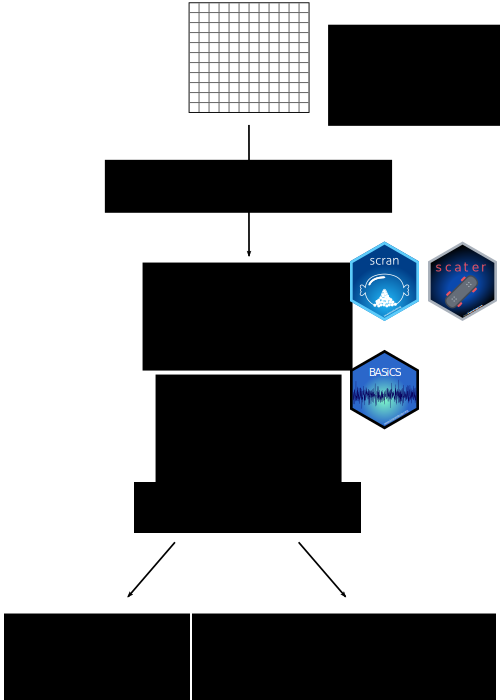
\includegraphics[width=0.5\linewidth]{figure/Overview} 

}

\caption{Graphical overview for the scRNA-seq analysis workflow described in this manuscript. Starting from a SingleCellExperiment object, we use the scater and scran Bioconductor packages to perform quality control and initial exploratory analyses. The primary focus of this workflow is to robustly quantify transcriptional heterogeneity within seemingly homogeneous cell populations. For this purpose, we apply the BASiCS Bioconductor package, illustrating how BASiCS can be used to analyse a single or multiple pre-specified groups of cells.}\label{fig:overview}
\end{figure}

\hypertarget{input-data---singlecellexperiment}{%
\subsection{\texorpdfstring{Input data - \texttt{SingleCellExperiment}}{Input data - SingleCellExperiment}}\label{input-data---singlecellexperiment}}

Here, we use the \emph{\href{https://bioconductor.org/packages/3.11/SingleCellExperiment}{SingleCellExperiment}} package to convert an input
matrix of raw read-counts (molecule counts for UMI-based protocols) into a
\texttt{SingleCellExperiment} object.
Such object can be used to store scRNA-seq data and its associated metadata,
such as gene- and cell-specific information.
Moreover, when available, the same object can be used to store read-counts for
technical spike-in molecules (these can be accessed via the \texttt{altExp()} method).
A major advantage of using a \texttt{SingleCellExperiment} object as the input for
scRNA-seq analyses is that it enables interoperability across a large number of
Bioconductor packages \citep{Amezquita2019}.

\hypertarget{quality-control-and-exploratory-analyses---scater-and-scran}{%
\subsection{\texorpdfstring{Quality control and exploratory analyses - \texttt{scater} and \texttt{scran}}{Quality control and exploratory analyses - scater and scran}}\label{quality-control-and-exploratory-analyses---scater-and-scran}}

An critical step in scRNA-seq analyses is to apply quality control (QC)
diagnostics, removing low quality samples (wells or droplets, depending on
the protocol) that may distort downstream analyses.
Among others, QC can help to identify samples that contain broken cells, that
are empty or that contain multiple cells \citep{Ilicic2016classification}.
Moreover, lowly expressed genes for which less reliable information is available
are typically also removed.

The \emph{\href{https://bioconductor.org/packages/3.11/scater}{scater}} Bioconductor package was developed to facilitate
this process \citep{McCarthy2017}.
It can be used to calculate standard QC metrics (e.g.~total reads per cell,
percentage of mitochondrial reads) and for data visualisation.\\
Here, we primarily use the \texttt{calculateQCMetrics} function to calculate cell-
and gene-specific QC metrics and the \texttt{plotPCA} function to visualise QC metrics,
exploring how these interact with available metadata.

The \emph{\href{https://bioconductor.org/packages/3.11/scran}{scran}} Bioconductor package offers a variety of functions
for low-level scRNA-seq data analysis \citep{Lun2016}.
While it contains function for doublet detection, and estimation
of cell cycle states, we will use it primarily for normalisation in conjunction
with the \texttt{scater} package \citep{Lun2016pooling}, and for modelling the mean-variance
trend across all genes. The \texttt{trendVar} and \texttt{decomposeVar} functions will be used to fit a
trend between the gene-specific variances and gene-specific mean expression,
before decomposing the overall variance into technical and biological
components. Furthermore, we will use the \texttt{DM} function to calculate the distance
of gene-specific squared coefficients of variation (CV\^{}2) to a rolling median
along mean expression \citep{Kolodziejczyk2015cell}.

\hypertarget{quantifying-cell-to-cell-transcriptional-variability---basics}{%
\subsection{\texorpdfstring{Quantifying cell-to-cell transcriptional variability - \texttt{BASiCS}}{Quantifying cell-to-cell transcriptional variability - BASiCS}}\label{quantifying-cell-to-cell-transcriptional-variability---basics}}

The \emph{\href{https://bioconductor.org/packages/3.11/BASiCS}{BASiCS}} Bioconductor package contains an assembly of
functions to estimate and analyse gene- and cell-specific model parameters
\citep{Vallejos2015BASiCS, Vallejos2016, Eling2018}.
\texttt{BASiCS} is build upon a hierarchical Baysian framework and as such samples
posterior distribution for each model parameter.
In mathematical terms, the gene expression count \(X_{ij}\) for gene \(i\) in cell
\(j\) is modelled as:

\[
\begin{aligned}
X_{ij}|\mu_i,\nu_j&\sim{}\text{Poisson}(\nu_j\mu_i)\\
\nu_j|s_j,\theta&\sim{}\text{Gamma}(1/\theta,1/(s_j\theta))\\
\rho_{ij}|\delta_i&\sim{}\text{Gamma}(1/\delta_i,1/\delta_i)
\end{aligned}
\]

where \(\mu_i\) explains the gene's mean expression, \(\nu_j\) the technical effect
characterised by the mRNA capture efficiency \(s_j\) and the unexplained technical
noise parameter \(\theta\).
Here, \(\rho_{ij}\) the biological
random effect fluctuating around the gene-specific over-dispersion
hyper-parameter \(\delta_i\).
It is important to note that, in further analyses, \(\mu_i\) represents the
mean expression and \(\delta_i\) the biological over-dispersion of each gene.

Due to a strong association between mean expression and biological
over-dispersion, the model has been extended to correct for such confounding
effect. To this end, the prior distribution for the over-dispersion parameters
has been changed to:

\[
\delta_i | \mu_i \sim \text{log-t}_{\eta}\left( \text{f}(\mu_i), \sigma^2 \right).
\]

where \(\text{f}(\mu_i)\) describes a smooth regression trend between the
over-dispersion and the mean expression parameters.
This extension introduced the residual over-dispersion parameters
\(\epsilon_i=\delta_i-\text{f}(\mu_i)\) that do not scale with mean expression
\citep{Eling2018}.

From a data analysis perspective, the \texttt{BASiCS\_MCMC} function is the heart of
the \texttt{BASiCS} package, and can be run in four different settings (see Table 1).

\begin{table}[htbp]
\caption{Four settings that can be used to run the \texttt{BASiCS\_MCMC} function.}
\centering
\begin{tabledata}{@{}lll@{}}
\header & No regression & Regression\\
\row Using spike-in reads & \texttt{WithSpikes\ =\ TRUE} & \texttt{WithSpikes\ =\ TRUE}\\
\row & \texttt{Regression\ =\ FALSE} & \texttt{Regression\ =\ TRUE}\\
\row No spike-ins available & \texttt{WithSpikes\ =\ FALSE} & \texttt{WithSpikes\ =\ FALSE}\\
\row & \texttt{Regression\ =\ FALSE} & \texttt{Regression\ =\ TRUE}\\
\end{tabledata}
\end{table}

If spike-in counts are availabe and should be used to estimate technical noise,
the parameter \texttt{WithSpikes} is set to \texttt{TRUE} (default).
If the regression between over-dispersion and mean expression should be
performed, the \texttt{Regression} parameters is set to \texttt{TRUE} (default).
If the user decides to set \texttt{Regression\ =\ FALSE}, \texttt{BASiCS} will not estimate
the regression trend, and will not supply the residual over-dispersion
parameters \(\epsilon_i\).

The \texttt{BASiCS\_MCMC} function returns a \texttt{BASiCS\_Chain} object, which can be used
for further downstream analyses, many of which are detailed in this workflow.
These objects contain draws from Markov chain Monte Carlo (MCMC) samplers,
which are used to infer the posterior distribution over the model parameters
\citep{Smith1993}.
Briefly, the posterior distribution quantifies how probable different parameter
values are given the observed data. However, before assessing the posterior
distribution, we must first ensure that the MCMC sampler has converged to
its stationary distribution, and has sampled efficiently from this distribution
\citep{Cowles1996}. If these conditions are not met, then the estimated parameters
may be inaccurate. The \emph{\href{https://CRAN.R-project.org/package=coda}{coda}} CRAN package contains a variety of
functions to assess the convergence of a sampled MCMC chain.
To use \texttt{coda} functions, the individual chains returned by \texttt{BASiCS} need to be
transformed into a MCMC object that \texttt{coda} recognises using the \texttt{coda::mcmc}
function. \texttt{BASiCS} also offers a number of functions to visualise and assess the
convergence of MCMC chains. In particular, we will use
\texttt{BASiCS\_EffectiveSize} and \texttt{BASiCS\_DiagPlot} to calculate and visualise the
effective sample size generated by the MCMC samplers.

\hypertarget{other-steps-title-tbc}{%
\subsection{Other steps {[}title tbc{]}}\label{other-steps-title-tbc}}

The \emph{\href{https://bioconductor.org/packages/3.11/goseq}{goseq}} Bioconductor package offers functions to detect the
enrichment of gene ontologies (GOs) among user-specified gene sets \citep{Young2010}.
Furthermore, \texttt{goseq} corrects for gene length biases, which is useful for full
length scRNA-seq data as highlighted in the first section.
In this workflow, we will use \texttt{goseq} to detect GO enrichment among
differentially expressed sets of genes.

For downstream analysis, such as GO enrichment analysis or the biological
interpretation of individual genes, we need to (i) link each gene's ID to its
symbol and (ii) calculate each gene's length.
For the first task, the \emph{\href{https://bioconductor.org/packages/3.11/biomaRt}{biomaRt}} Bioconductor package annotates a
wide range of gene and gene product identifiers \citep{Durinck2005} by accessing the
BioMart software suite (\url{http://www.biomart.org}).
We can use \texttt{biomaRt} to link the \textbf{Mus musculus} gene IDs and to their gene
symbols (also referred to as `gene name'):

{\small\bibliography{Workflow.bib}}

\end{document}
